\noindent \textit{This chapter was originally published in collaboration with David C. Catling, Kevin J. Zahnle and Mark W. Claire in the Proceedings of the National Academy of Sciences \citep{Wogan_2022}, and is reproduced below with the permission of the journal.}

\section*{\centering Summary}

The Great Oxidation Event (GOE), arguably the most important event to occur on Earth since the origin of life, marks the time when an oxygen-rich atmosphere first appeared. However, it is not known whether the change was abrupt and permanent or fitful and drawn out over tens or hundreds of millions of years. Here, we developed a 1-D time-dependent photochemical model to resolve time-dependent behavior of the chemically unstable transitional atmosphere as it responded to changes in biogenic forcing. When forced with step-wise changes in biogenic fluxes, transitions between anoxic and oxic atmospheres take between only $10^2$ and $10^5$ years. Results also suggest that O$_2$ between $\sim10^{-8}$ and $\sim10^{-4}$ mixing ratio is unstable to plausible atmospheric perturbations. For example, when atmospheres with these O$_2$ concentrations experience fractional variations in the surface CH$_4$ flux comparable to those caused by modern Milankovitch cycling, oxygen fluctuates between anoxic ($\sim10^{-8}$) and oxic ($\sim10^{-4}$) mixing ratios. Overall, our simulations are consistent with possible geologic evidence of unstable atmospheric O$_2$, after initial oxygenation, which could occasionally collapse from changes in biospheric or volcanic fluxes. Additionally, modeling favors mid-Proterozoic O$_2$ exceeding $10^{-4}$ - $10^{-3}$ mixing ratio, otherwise O$_2$ would periodically fall below $10^{-7}$ mixing ratio, which would be inconsistent with post-GOE absence of sulfur isotope mass-independent fractionation.

\section{Introduction}

Abundant atmospheric O$_2$ at 21\% by volume is the most distinctive and consequential feature of Earth's atmosphere. Produced by cyanobacteria, algae and plants, O$_2$ is a clear sign of our biosphere that is detectable across interstellar space by telescopic spectroscopy \citep{Meadows_2018}. Oxygen permits aerobic respiration, the only known metabolism  with sufficient energy yield that can sustain complex animal life \citep{Catling_2005}. However, for about the first half of Earth's 4.5-billion-year-old history, the atmosphere had negligible O$_2$ \citep[e.g.][]{Catling_2020}. This changed $\sim$2.4 billion years ago.

The timing of the GOE, and magnitude of atmospheric O$_2$ concentrations before and after the GOE can be constrained by the geologic record of sulfur isotopes in combination with photochemical models. Archean and earliest Proterozoic sedimentary minerals contain sulfur isotopes with characteristic mass independent fractionation (MIF) which abruptly disappears 2.4 billion years ago \citep{Warke_2020}. Sulfur MIF in marine sediments likely requires that atmospheric photochemistry produce elemental sulfur, S$_8$ \citep[for explanation, see the introduction in][]{Zahnle_2006} \citep{Pavlov_2002,Farquhar_2000}. \citet{Zahnle_2006} used a 1-D photochemical model to show that atmospheric S$_8$ production only occurs when atmospheric O$_2$ is below $\sim 2 \times 10^{-7}$ mixing ratio. An often cited threshold of $2 \times 10^{-6}$ was from an earlier photochemical model that did not simulate atmospheres with surface O$_2$ mixing ratios between $2 \times 10^{-6}$ and $\sim 10^{-15}$ \citep{Pavlov_2002}. Therefore, the disappearance of the sulfur isotope MIF signal at 2.4 Ga is strong evidence that O$_2$ first rose above $2 \times 10^{-7}$ mixing ratio.

Geologic evidence may suggest that the GOE was not a single monotonic rise of oxygen but characterized by oscillations. Using U-Pb dating, \citet{Gumsley_2017} updated the chronology of sulfur isotope MIF in the stratigraphic record, finding evidence for two oxic-to-anoxic transitions between $\sim 2.4$ and $\sim 2.3$ Ga. More recently, \citet{Poulton_2021} report 2.3 - 2.2 Ga marine sediments with sulfur isotopes consistent with approximately five oxic-to-anoxic transitions. Fluctuating O$_2$ levels coincide with three to four widespread glaciations, indicating extreme climate instability \citep{Rasmussen_2013}. Overall, geochemical evidence tentatively suggests that O$_2$ concentrations and climate were unstable for 200 million years until $\sim 2.2$ Ga, which marks the most recent estimated timing of the permanent oxygenation of the atmosphere \citep{Poulton_2021}. However, interpretations of oscillating O$_2$ have been questioned \citep{Izon_2022}. While the geologic evidence for the O$_2$ oscillations remains equivocal, the data has raised significant questions regarding the feasibility and timescales for Earth's great oxidation. Some have argued that the oxygen-rich atmosphere is more stable than an oxygen-poor atmosphere \citep{Goldblatt_2006}, which favors a single rise of O$_2$ instead of O$_2$ oscillations.

Evidence for O$_2$ instability and the time-dependent behavior of O$_2$ concentrations have not been reconciled with atmospheric photochemical models. All previous models treated the GOE as successive photochemical steady states \citep{Kasting_1980,Segura_2003,Pavlov_2001,Pavlov_2002,Zahnle_2006,Bethan_2021,Claire_2014,Izon_2017,Kurzweil_2013}. A photochemical steady state occurs when no atmospheric species changes concentration over time because their production and loss from reactions and surface sources (e.g. volcanoes or biology) are balanced. Such steady state calculations have been crucial for understanding the GOE by contextualizing sulfur isotope MIF observations \citep{Pavlov_2002,Zahnle_2006}, and establishing the relationship between atmospheric O$_2$ concentrations and the degree to which O$_3$ blocks UV photons from Earth's surface (i.e. O$_3$ shielding) \citep{Kasting_1980,Pavlov_2001,Bethan_2021}, but they do not evaluate time-dependent changes and transient imbalances, or characteristic timescales.

Several theories for the rise of O$_2$ suggest that it relied on a global redox titration over $10^8$ - $10^9$ years involving oxidation of the upper mantle and/or crust, plausibly driven by hydrogen escape, which led to a tipping point where the source flux of O$_2$ exceeded a kinetically rapid O$_2$ sink from volcanic and metamorphic reductants \citep{Catling_2001,Claire_2006,Kadoya_2020,Holland_2002,Kasting_1993}. Beyond the tipping point, O$_2$ flooded the atmosphere, reaching a new, long-term balance limited by oxidative weathering. 

Here, we developed a novel, time-dependent 1-D photochemical model capable of investigating changes of O$_2$ at the tipping point itself over timescales $10^2$ - $10^5$ years rather than the longer-term planetary changes which initiated the GOE. We simulate changing O$_2$ as a time-dependent evolution, in contrast to the steady-state approach used in previous studies \citep[e.g.][]{Kasting_1980}, because O$_2$ can change on relatively rapid timescales that are not well characterized by steady-states. With our model, we compute the time required for an anoxic-to-oxic atmospheric transition, and the time required for de-oxygenation. Additionally, we investigate the stability of O$_2$ concentrations against perturbations to surface gas fluxes produced by biology. Finally, we use our model results to better constrain O$_2$ levels and stability during the GOE (starting $\sim 2.4$ Ga), and during the mid-Proterozoic eon (1.8 to 0.8 Ga).

\section{Methods}

To investigate the transition between an anoxic and oxygen rich Earth, we use a photochemical model with one spatial dimension of altitude, approximating a global average vertical profile. One-dimensional photochemical models are typically governed by a simplification of the continuity equation for molecules:

\begin{equation} \label{eq:continuity}
  \frac{\partial n_{i}}{\partial t} = - \frac{\partial}{\partial z}\Phi_{i} + P_{i} - L_{i} + R_{\text{i,\ rainout}} + Q_{\text{i,\ lightning}}
\end{equation}
Table \ref{tab:variables} defines all the variables and their units. Here, the flux ($\Phi_{i}$) is given by

\begin{equation} 
  \Phi_{i} = - Kn\frac{\partial}{\partial z}\left( \frac{n_{i}}{n} \right) - D_{i}n_{i}\left( \frac{1}{n_{i}}\frac{\partial n_{i}}{\partial z} + \frac{1}{H_{i}} + \frac{1 + \alpha_{\text{Ti}}}{T}\frac{\partial T}{\partial z} \right)
\end{equation}
The above system of partial differential equations (PDEs) describes how the number density ($n_{i}$) of each chemical species $i$ changes over altitude and time.

In our photochemical model, we solve a simplified version of Equation \eqref{eq:continuity} which assumes that the total number density does not change over time ($\partial n / \partial t \approx 0$). This assumption is valid for atmospheric transitions which maintain approximately constant surface pressure and atmospheric temperature. The continuity equations can then be written in terms of mixing ratios ($f_{i}$) instead of number densities (see Appendix B.1 in \citet{Catling_2017} for a derivation):

\begin{equation} \label{eq:continuity_simple}
  \frac{\partial f_{i}}{\partial t} = - \frac{1}{n}\frac{\partial}{\partial z}\Phi_{i} + \frac{P_{i}}{n} - \frac{L_{i}}{n} - \frac{R_{\text{i,\ rainout}}}{n} + \frac{Q_{\text{i,\ lightning}}}{n}
\end{equation}

\begin{equation}
  \Phi_{i} = - \left( K + D_{i} \right)n\frac{\partial f_{i}}{\partial z} - \zeta_{i}nf_{i}
\end{equation}

\begin{equation}
  \zeta_{i} = D_{i}\left( \frac{1}{H_{i}} - \frac{1}{H_{a}} + \frac{\alpha_{\text{Ti}}}{T}\frac{\partial T}{\partial z} \right)
\end{equation}

\begin{table}
\caption{Variables in Equation \eqref{eq:continuity}}
\label{tab:variables}
\centering
\begin{tabularx}{0.85\textwidth}{p{0.15\linewidth} | p{0.4\linewidth} | p{0.3\linewidth}}
\hline \hline
Variable & Definition & Units \\
\hline
\(f_{i}\) & Mixing ratio of species \(i\) & dimensionless \\
\(n_{i}\) & Number density of species \(i\) & molecules
cm\textsuperscript{-3} \\
\(z\) & Altitude & cm \\
\(t\) & Time & seconds \\
\(n\) & Total number density & molecules
cm\textsuperscript{-3} \\
\(P_{i}\) & Total chemical production of species \(i\) & molecules
cm\textsuperscript{-3} s\textsuperscript{-1} \\
\(L_{i}\) & Total chemical loss of species \(i\) & molecules
cm\textsuperscript{-3} s\textsuperscript{-1} \\
\(R_{\text{i, rainout}}\) & Production and loss of species \(i\) from
rainout & molecules cm\textsuperscript{-3}
s\textsuperscript{-1} \\
\(Q_{\text{i, lightning}}\) & Production and loss of species \(i\)
from lightning & molecules cm\textsuperscript{-3}
s\textsuperscript{-1} \\
\(\Phi_{i}\) & Vertical flux of species \(i\) & molecules
cm\textsuperscript{-2} s\textsuperscript{-1} \\
\(K\) & Eddy diffusion coefficient & cm\textsuperscript{2}
s\textsuperscript{-1} \\
\(D_{i}\) & Molecular diffusion coefficient & cm\textsuperscript{2}
s\textsuperscript{-1} \\
\(H_{i}\) & \(= N_{a}\text{kT}\text{/}\mu_{i}g\), The scale heights of
species \(i\) & cm \\
\(H_{a}\) & \(= N_{a}\text{kT}\text{/}\overline{\mu}g\), The average
scale height. & cm \\
\(N_{a}\) & Avogadro's number & molecules
mol\textsuperscript{-1} \\
\(k\) & Boltzmann's constant & erg K\textsuperscript{-1} \\
\(\mu\) & Molar mass. \(\overline{\mu}\) is mean molar mass of the
atmosphere, and \(\mu_{i}\) is the molar mass of species \(i\) & g
mol\textsuperscript{-1} \\
\(g\) & Gravitational acceleration & cm
s\textsuperscript{-2} \\
\(\alpha_{\text{Ti}}\) & Thermal diffusion coefficient of species \(i\).
We neglect this term (\(\alpha_{\text{Ti}} = 0\)) &
dimensionless \\
\(T\) & Temperature & K \\
\end{tabularx}
\end{table}

To approximate Equation \eqref{eq:continuity_simple}, the model replaces the spatial derivatives with finite difference approximations, turning the system of PDEs into a larger system of ordinary differential equations (ODEs). This is the ``method of lines'' approach to solving a PDE. \citet{Catling_2017}, their Appendix B.2, provides a detailed description of how to do this with Equation \eqref{eq:continuity_simple}, therefore we will omit a detailed description here, except to point out a sign error. The first two terms for the equation for $B$ in their equation B.16 should have minus signs instead of plus signs.

The system of ODEs derived from finite differencing Equation \eqref{eq:continuity_simple} can be evolved forward in time with numerical integration. However, the photochemical ODEs are ``stiff'', meaning that some dependent variables (i.e. the mixing ratios) change much more quickly than others. For example, in the modern atmosphere, OH typically has a chemical lifetime of about 1 second, while CH\textsubscript{4} has a chemical lifetime of ${\sim}10$ years. Stiff equations require special, high stability, ``implicit'' integration methods. For more details on stiff equations and the implicit methods used to solve them, see \citet{Hairer_1996}.

Often, we solve for steady states of the photochemical continuity equation ($\frac{\partial f_{i}}{\partial t} = 0$). To find steady states, we begin with some initial atmospheric composition, then integrate Equation \eqref{eq:continuity_simple} forward in time until the atmosphere ceases to change, i.e. a steady state is reached. The assumption of photochemical steady state is approximately valid for most periods of Earth's history because the atmosphere changes slowly enough to be in a quasi-steady state.

However, the Paleoproterozoic rise of O$_2$ was a relatively fast atmospheric transition that is not well modeled as a photochemical steady state process. Therefore, describing it requires accurately solving the continuity equation over time.

To model the photochemistry of the GOE, we modified the photochemical model contained within the \textit{Atmos} modeling suite (described in Appendix B of \citet{Catling_2017}) so that it can accurately solve the time dependent behavior of Equation \eqref{eq:continuity_simple}. We call the modified version of the model PhotochemPy. Instead of using a Backward Euler as in \textit{Atmos}, we used CVODE BDF ODE solver from Sundials Computing \citep{Hindmarsh_2005}. CVODE BDF is an implementation of the backward differential formulas (BDF) and is a gold-standard for solving large chemical kinetics problems. For details, see Section \ref{sec:goe_appendix}.

PhotochemPy is open source under an MIT license. The version of the code (v0.2.14) used in this paper and the corresponding Python scripts to reproduce work done in this article is at \url{https://doi.org/10.5281/zenodo.6824092}. However, the most up to date version of the code can be found at the following Github link: \url{https://github.com/Nicholaswogan/PhotochemPy}.

\section{Results} \label{sec:goe_results}

\begin{figure}
  \centering
  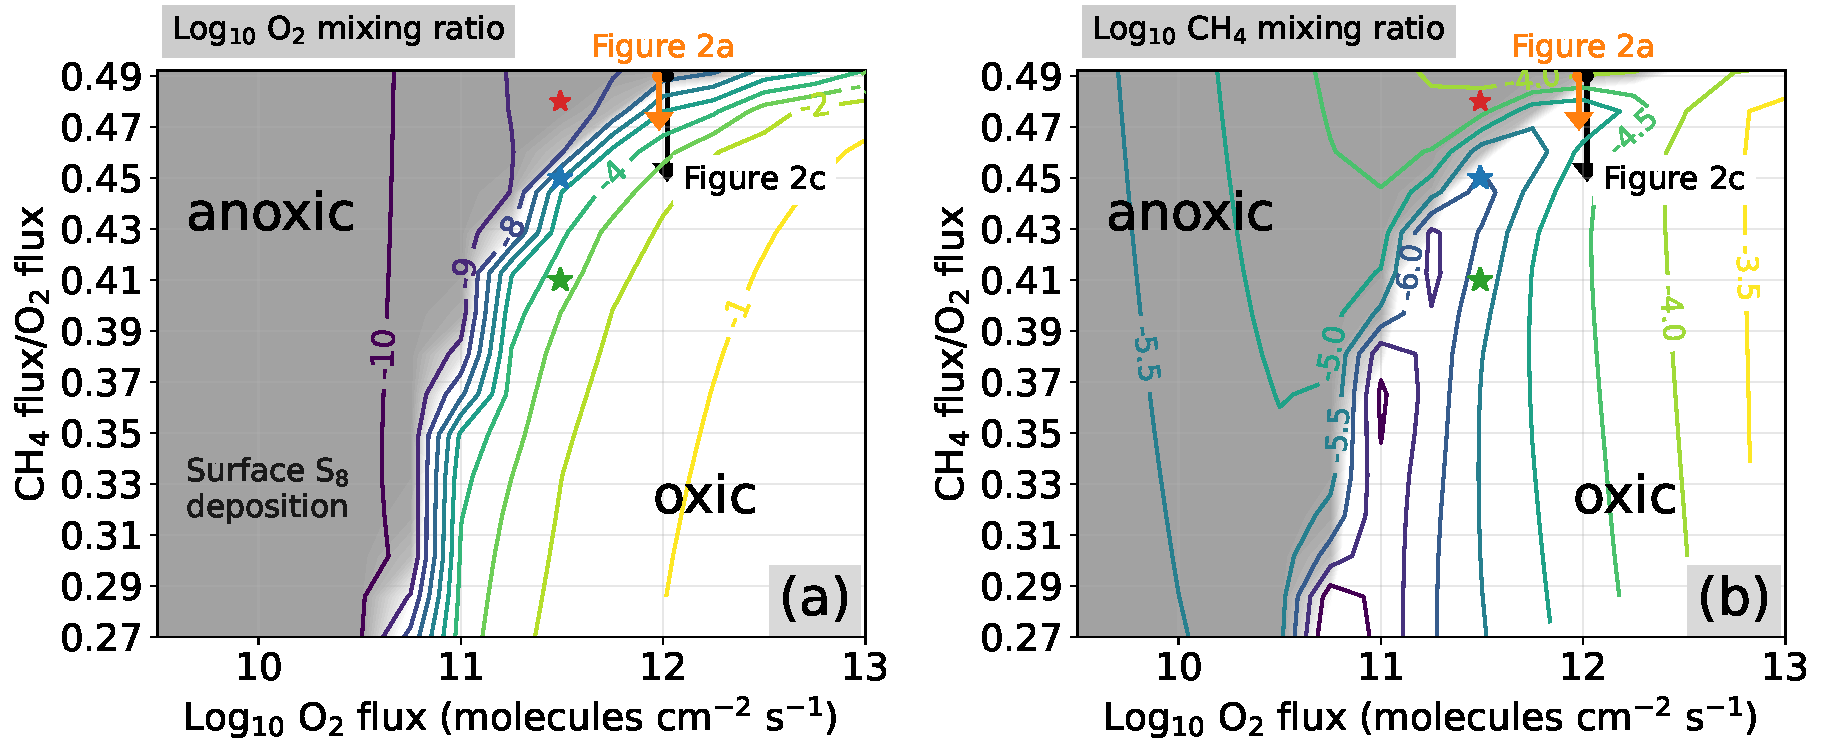
\includegraphics[width=\textwidth]{tex/4goe/main/ArcheanOutgassing_sweep.pdf}
  \caption{Colored contours show photochemical steady states of (a) $\log_{10}$ surface O$_2$ mixing ratio, and (b) $\log_{10}$ surface CH$_4$ mixing ratio as a function of $\log_{10}$ O$_2$ surface flux and CH$_4$ flux / O$_2$ flux. Grey shading indicates the magnitude of elemental S$_8$ production in the atmosphere, which is considered essential for the preservation of sulfur isotope mass independent fractionation in marine sediments. Peak S$_8$ production is $\sim10^7$ molecules cm$^{-2}$ s$^{-1}$. Grey shading fades to white for S$_8$ production less than $10^{-10}$ molecules cm$^{-2}$ s$^{-1}$, a negligibly small value. Arrows labeled ``Figure \ref{fig:oxygenation}a" and ``Figure \ref{fig:oxygenation}c" indicate start and endpoints for time-dependent photochemical models of the oxic transition shown in Figures \ref{fig:oxygenation}a and \ref{fig:oxygenation}c. Red, blue and green stars are the initial conditions used in the simulations shown in Figures \ref{fig:stability}b, \ref{fig:stability}c, and \ref{fig:stability}d, respectfully.}
  \label{fig:sweep}
\end{figure}

\begin{table}
  \caption{Fixed surface flux boundary conditions for SO$_2$, H$_2$S, H$_2$, and CO used in this study. All fluxes have units of molecules cm$^{-2}$ s$^{-1}$}
  \label{tab:volc_fluxes}
  \centering
  \begin{tabularx}{\linewidth}{p{0.15\linewidth}  p{0.17\linewidth} p{0.17\linewidth}  p{0.17\linewidth}  p{0.17\linewidth}}
  \hline \hline
  Model & SO$_2$ & H$_2$S & H$_2$ & CO \\
  \hline
  Archean Outgassing$\mathrm{^a}$ &$10^{10}$& $10^{9}$ & $3\times 10^{10}$ & $3\times 10^{9}$\\
  Modern Values$\mathrm{^b}$ &$3.5\times10^{9}$& $3.5\times10^{8}$ & $1.22\times 10^{8}$ & $2.65\times 10^{11}$\\
  \hline
  \multicolumn{5}{>{\raggedright\arraybackslash}p{0.95\linewidth}}{$\mathrm{^a}$ The same fluxes as the ``Archean High'' values from Table 1 in \citet{Zahnle_2006}.

  $\mathrm{^b}$ Surface flux values required to reproduce the concentration of each gas in the modern Earth's atmosphere. These values are also the ``Case 1'' fluxes described in \citet{Bethan_2021}.} 
  \end{tabularx}
\end{table}

To investigate the time-dependent behavior of O$_2$ during the GOE, we first computed grids of photochemical steady state atmospheres. These steady states establish context for time-dependent photochemical modeling described in subsequent sections. Figure 1 shows predicted steady state surface O$_2$ mixing ratio (Figure \ref{fig:sweep}a), surface CH$_4$ mixing ratio (Figure \ref{fig:sweep}b), and the precipitation of atmospheric S$_8$ (gray shading) as a function of surface O$_2$ flux between $3 \times 10^{9}$ and $10^{13}$ molecules cm$^{-2}$ s$^{-1}$, and CH$_4$ flux / O$_2$ flux ratios between 0.27 to 0.49 where gas fluxes are those entering the atmosphere. The surface O$_2$ fluxes reported here are net emissions into the atmosphere which exclude recycling within the biosphere. For reference, a comparable model of the modern Earth requires a surface O$_2$ flux of $10^{12}$ molecules cm$^{-2}$ s$^{-1}$, and a CH$_4$ flux / O$_2$ flux of 0.09 (CH$_4$ flux = $\sim9 \times 10^{10}$ molecules cm$^{-2}$ s$^{-1}$) \citep{Bethan_2021}. We consider a CH$_4$ flux / O$_2$ flux ratio close to 0.5 to be more realistic for the late Archean, prior to the GOE, because this ratio is expected if oxygenic photosynthesis is balanced by methanogenesis. In net \citep{Claire_2006}, where ``CH$_2$O'' represents organic matter:

\begin{equation}
\begin{aligned}
    \mathrm{CO_2} + \mathrm{H_2O} \rightarrow \mathrm{CH_2O} + \mathrm{O_2} \quad\quad &\text{(Oxygenic Photosynthesis)} \\
    2 \mathrm{CH_2O} \rightarrow \mathrm{CH_4} + \mathrm{CO_2} \quad\quad &\text{(Methanogenesis)} \\
    \mathrm{CO_2} + 2\mathrm{H_2O} \rightarrow \mathrm{CH_4} + 2 \mathrm{O_2} \quad\quad &\text{(Net)}
\end{aligned}
\end{equation}
The CH$_4$ flux / O$_2$ flux ratio is smaller than 0.5 on the modern Earth largely because of the microbial anerobic oxidation of methane via $\mathrm{SO_4^{2-}}$ in ocean sediments, a process that was unimportant in the anoxic mid-Archean ocean with little sulfate \citep{Canfield_2000,Catling_2007,Olson_2016}. We include O$_2$ fluxes several orders of magnitude smaller than the modern value ($\sim 10^{12}$ molecules cm$^{-2}$ s$^{-1}$) because of evidence for smaller primary productivity during the Proterozoic eon \citep{Laakso_2019,Kipp_2021}.

Recall that atmospheric S$_8$ deposition is considered necessary to preserve sulfur isotope MIF in ocean sediments \citep{Pavlov_2002}. We find that S$_8$ production is not possible above $\sim10^{-7}$ O$_2$ mixing ratio (the gray-to-white shading boundary in Figure \ref{fig:sweep}), consistent with previous results \citep{Zahnle_2006}.

Figure \ref{fig:sweep} uses Archean outgassing surface fluxes for CO, H$_2$, H$_2$S, and SO$_2$ listed in Table \ref{tab:volc_fluxes}, with the CO$_2$ surface mixing ratio fixed to 1\% for all model runs - a reasonable value for the late Archean according to carbon cycle modeling \citep{KrissansenTotton_2018_carbon}. Additionally, over the same span of surface O$_2$ fluxes and H$_2$ flux / O$_2$ flux ratios, we compute photochemical steady states for the modern fluxes for CO, CH$_4$, H$_2$S, and SO$_2$ listed in Table \ref{tab:volc_fluxes}, again fixing CO$_2$ to 1\%. The results are shown in Figure \ref{fig:case1} in Section \ref{sec:goe_appendix}.

In the following sections, we calculate the time required to transition between different steady state atmospheres shown in Figures \ref{fig:sweep} and \ref{fig:case1}.

\subsection{The timescale of atmospheric oxygenation} \label{sec:oxygenation}

\begin{figure}
  \centering
  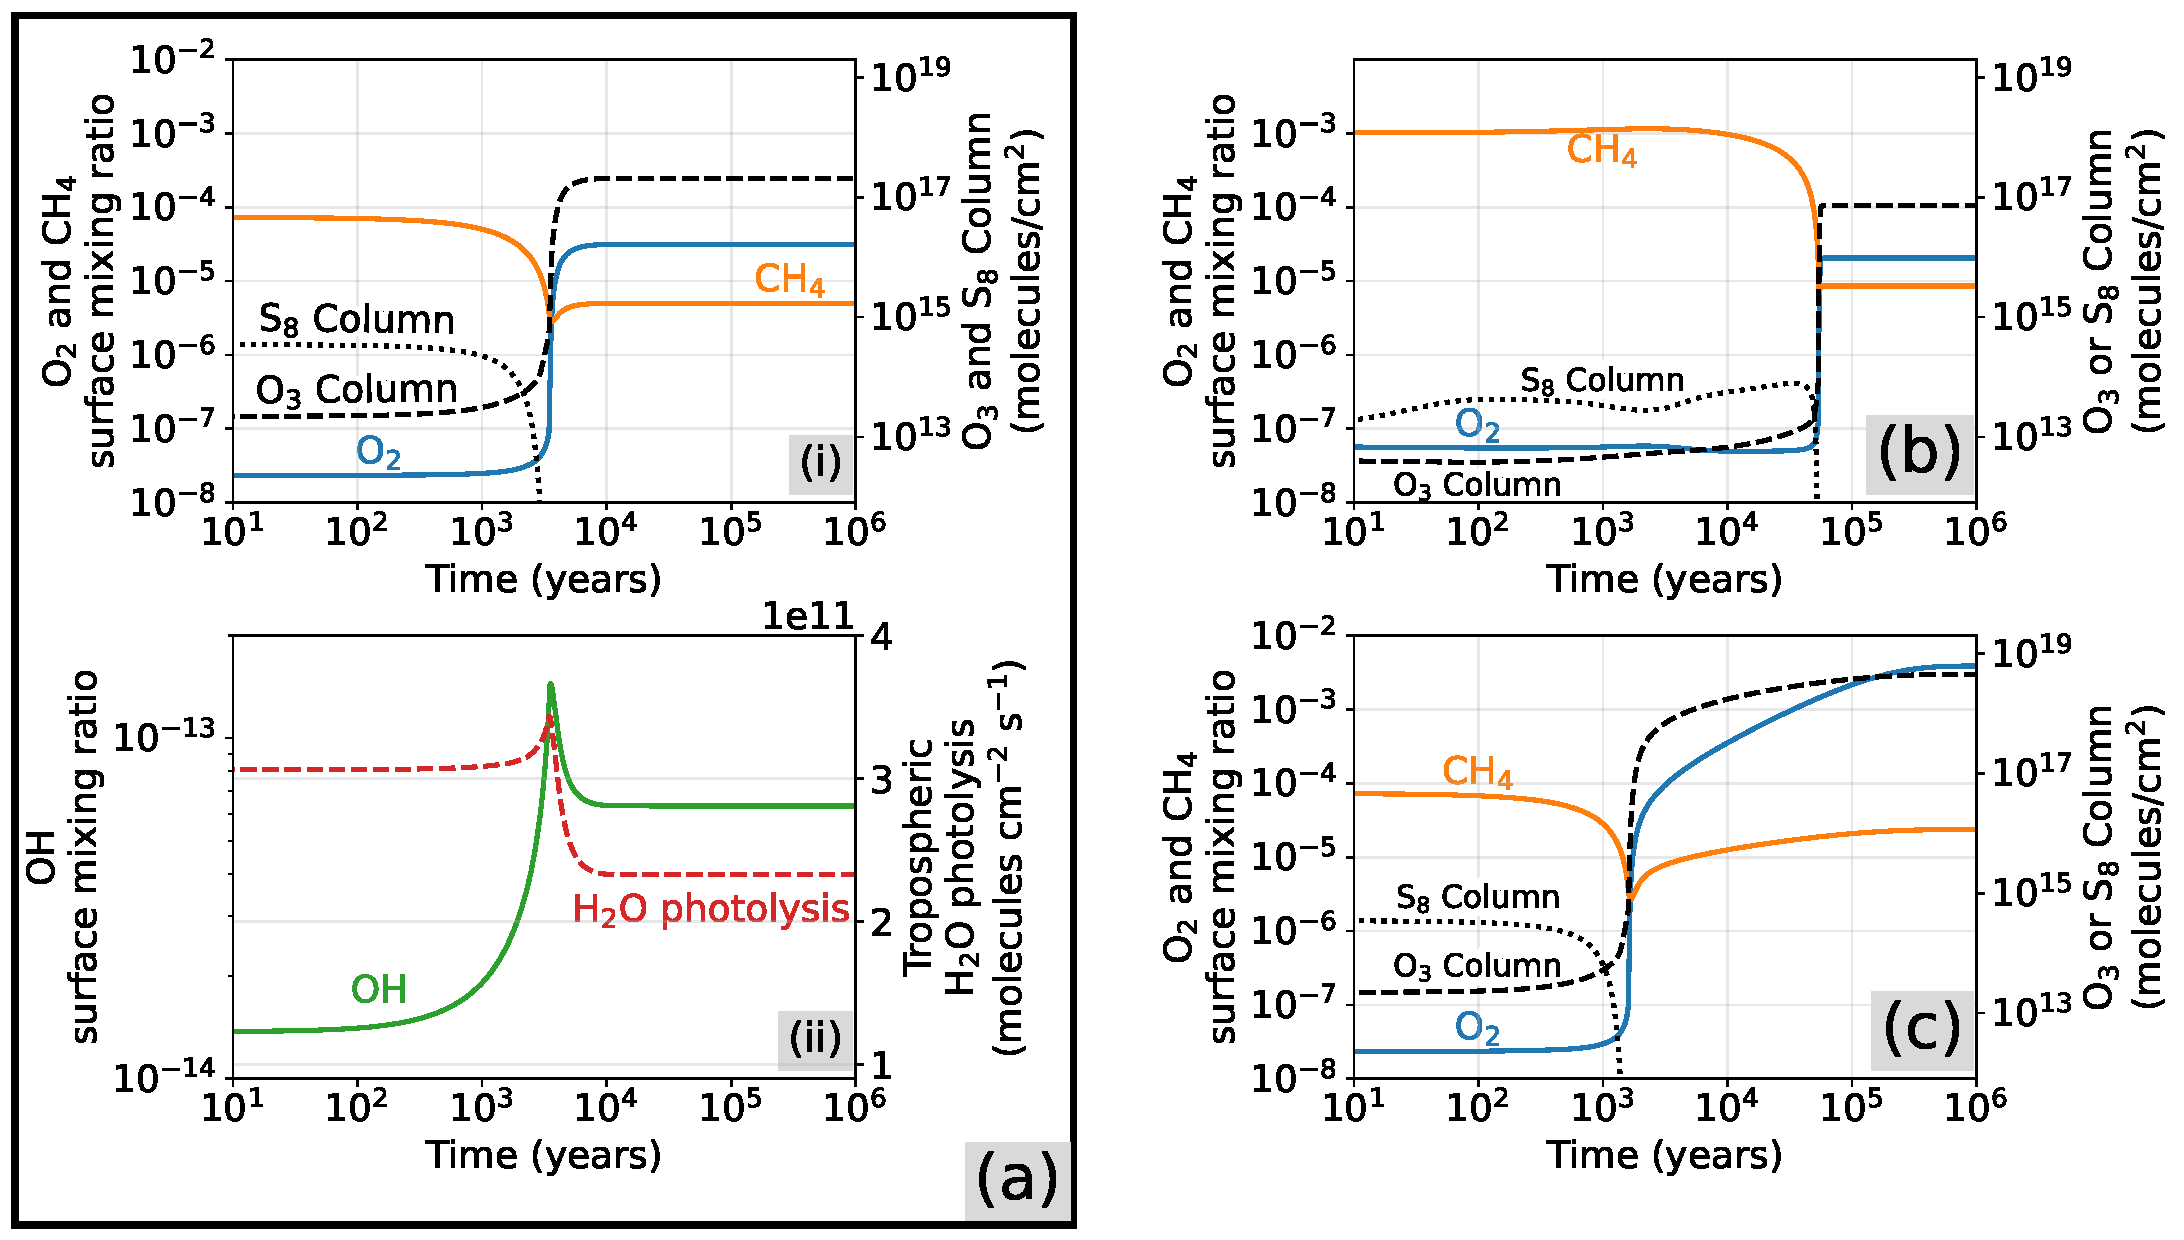
\includegraphics[width=\textwidth]{tex/4goe/main/Oxygenation.pdf}
  \caption{Three models of anoxic to oxic transitions. (a) Shows atmospheric oxygenation caused by a step-wise decrease in the methane flux from $4.9 \times 10^{11}$ to $4.7 \times 10^{11}$ molecules cm$^{-2}$ s$^{-1}$ (orange arrow in Figure \ref{fig:sweep}). Panel (i) shows surface O$_2$ and CH$_4$ mixing ratios, and O$_3$ and S$_8$ column abundance over time; Panel (ii) shows OH surface mixing ratio and tropospheric H$_2$O photolysis rate. (b) Shows transition caused by step-wise increase in the O$_2$ flux from $10^{12}$ to $1.8 \times 10^{12}$ molecules cm$^{-2}$ s$^{-1}$ and a stepwise increase in the CH$_4$ flux to maintain constant CH$_4$ flux / O$_2$ flux = 0.45 (Figure \ref{fig:case1}). Transition in (c) results from a step-wise decrease in the CH$_4$ flux from $4.9 \times 10^{11}$ to $4.5 \times 10^{11}$ molecules cm$^{-2}$ s$^{-1}$ (black arrow in Figure \ref{fig:sweep}).}
  \label{fig:oxygenation}
\end{figure}

The orange arrow labeled ``Figure \ref{fig:oxygenation}a'' in Figure \ref{fig:sweep} corresponds to the approximate start and end states of the time-dependent photochemical model run shown in Figure \ref{fig:oxygenation}a. The model starts with an atmosphere at a steady state, then at $t = 0$ years, we impose a stepwise decrease in the surface methane flux from $4.9 \times 10^{11}$ to $4.7 \times 10^{11}$ molecules cm$^{-2}$ s$^{-1}$ (we keep the surface O$_2$ flux constant at $10^{12}$ molecules cm$^{-2}$ s$^{-1}$). This perturbation causes O$_2$ to rise from $3 \times 10^{-8}$ to $3 \times 10^{-5}$ mixing ratio over $\sim 3500$ years, eliminating photochemical S$_8$ production. 

The O$_2$ transition in Figure \ref{fig:oxygenation}a(i) is modulated by O$_3$ shielding of tropospheric H$_2$O \citep{Kasting_1980}. When a stratospheric O$_3$ layer begins to develop, OH production from H$_2$O decreases (Figure \ref{fig:oxygenation}a(ii)). Decreasing OH concentrations prevent the mutual annihilation of O$_2$ and CH$_4$ (by $\mathrm{CH_4} + \mathrm{OH} \rightarrow \mathrm{CH_3} + \mathrm{H_2O}$ followed by $\mathrm{CH_3} + \mathrm{O_2} \rightarrow \text{products}$), so O$_2$ levels increase. The mixing ratio of CH$_4$ also rebounds. O$_3$ shielding (protecting life on the surface from harmful solar UV radiation) is just barely beginning to operate in this example compared to the modern Earth. After the atmosphere reaches a new steady state, the atmospheric column has $3 \times 10^{17}$ O$_3$ molecules cm$^{-2}$, some $26$ times smaller than the modern value of $8 \times 10^{18}$ molecules cm$^{-2}$. Note, the extent to which O$_3$ shields tropospheric H$_2$O can be strongly modulated by 3-D dynamical effects \citep{Cooke_2022}, which we do not account for.

Like Figure \ref{fig:oxygenation}a, Figure \ref{fig:oxygenation}b also shows a transition between $5 \times 10^{-8}$ and $2 \times 10^{-5}$ O$_2$ mixing ratio, but this model uses the modern outgassing fluxes for CO, H$_2$, H$_2$S, and SO$_2$ listed in Table \ref{tab:volc_fluxes} instead of presumptive Archean outgassing values. Also, at $t = 0$ years, we impose a stepwise increase of the O$_2$ flux from $10^{12}$ to $1.8 \times 10^{12}$ molecules cm$^{-2}$ s$^{-1}$ while keeping the CH$_4$ flux / O$_2$ flux ratio at 0.45 (see Figure \ref{fig:case1} for context). While the anxoic-to-oxic transition itself still occurs rapidly, the atmosphere simulated in Figure \ref{fig:oxygenation}b takes 60,000 years to reach the tipping point, which is much longer than the comparable O$_2$ transition shown in Figure \ref{fig:oxygenation}a.

The time required for O$_2$ to begin to rise in concentration is controlled by the reservoir of reducing gases, primarily CH$_4$, H$_2$ and CO, in the pre-oxygenated atmosphere. Big reservoirs of reducing gases slow the timescale of oxygenation because reducing gases must be mostly removed before O$_2$ can increase. O$_2$ cannot increase while reducing gases are abundant because large oxygen sinks from reactions with reducing gases prevent it. That is why 3,500 years elapse before O$_2$ begins to rise in Figure \ref{fig:oxygenation}a, and why 60,000 years elapse before O$_2$ rises in Figure \ref{fig:oxygenation}b. Figure \ref{fig:oxygenation}b starts with more reducing gases, which take longer to eradicate.

We can roughly estimate the time required for O$_2$ to begin to rise with a back-of-the-envelope calculation of the rate that reducing gases are eliminated from the anoxic atmosphere. The total reservoir of reducing gases in the pre-oxygenated atmosphere in O-equivalent units is

\begin{equation} 
  N_\mathrm{reducing} = \sum_j N_j \alpha_j \approx -4 N_\mathrm{CH_4} - N_\mathrm{CO} - N_\mathrm{H_2} 
\end{equation}
Here, $N_\mathrm{reducing}$ is the O-equivalent column abundance of reducing gases (O$_\mathrm{equiv}$ molecules cm$^{-2}$), which is equal to the sum of all reducing gases in the atmosphere ($N_j$) multiplied by $\alpha_j$, the redox state of each gas. Redox state is a relative quantity that requires defining redox-neutral reference species. Following previous models of the early Earth \citep{Zahnle_2006}, we define H$_2$O, SO$_2$, CO$_2$ and N$_2$ as redox-neutral, with the oxygen redox parameter $\alpha_\mathrm{O} = +1$. Therefore, $\alpha_\mathrm{H} = -0.5$, $\alpha_\mathrm{S} = -2$, and $\alpha_\mathrm{C} = -2$, from redox stoichiometry of hydrogen, sulfur and carbon, respectfully. It then becomes straight-forward to calculate the $\alpha_j$ for any molecule. For example, $\alpha_\mathrm{CH_4} = \alpha_\mathrm{C} + 4\alpha_\mathrm{H} = -2 - 2 = - 4$. For a more in-depth explanation of atmospheric redox, see Section 3 in \citet{Harman_2015} or Chapter 8 in Catling and \citet{Catling_2017}. $N_\mathrm{reducing}$ is approximately equal to the weighted sum of CH$_4$, H$_2$, and CO because these are the main reducing gases in an Archean Earth-like atmosphere.

The change in column abundance of reducing gases is the difference between the redox columns at the finial and initial atmospheric states.

\begin{equation} 
  \Delta N_\mathrm{reducing} = N_\mathrm{reducing}^\text{final} - N_\mathrm{reducing}^\text{initial}
\end{equation}
In Figures \ref{fig:oxygenation}a and \ref{fig:oxygenation}b, we initiate the rise of oxygen by changing the surface flux of CH$_4$ and/or O$_2$ flux. We can quantify this flux perturbation in units of O$_\mathrm{equiv}$ molecules cm$^{-2}$ s$^{-1}$ ($\Delta F_\mathrm{O_{equiv}}$):

\begin{equation}
\begin{split}
  \Delta F_\mathrm{O_{equiv}} &= \sum_i F_i^\text{final} \alpha_i - \sum_i F_i^\text{initial} \alpha_i \\ 
  &= (2 F_\mathrm{O_2}^\text{final} - 4 F_\mathrm{CH_4}^\text{final}) - (2 F_\mathrm{O_2}^\text{initial} - 4 F_\mathrm{CH_4}^\text{initial})
\end{split}
\end{equation}
Therefore, the time required to oxidize the reducing gases in the atmosphere and permit oxygen to begin rising is approximately

\begin{equation} \label{eq:tau_oxy}
  \tau_\text{oxy} = \left| \frac{\Delta N_\text{reducing}}{\Delta F_\mathrm{O_{equiv}}} \right|
\end{equation}

Plugging in values for the O$_2$ transition in Figure \ref{fig:oxygenation}b yields $\tau_\text{oxy}=$ 2,900 years, a value only slightly smaller than the 3,500 years predicted by the time-dependent photochemical model. For Figure \ref{fig:oxygenation}b, $\tau_\text{oxy}=$ 29,000 years, which is about a factor of 2 smaller than the figure from 1-D photochemistry. Our estimate is too small in this case because the reducing column and its destruction rate is not constant prior to the rise of oxygen (see Section \ref{sec:goe_appendix}). This calculation illustrates that the time required for oxygen to begin rising, once a tipping point of fluxes is reached, mostly depends on the quantity of reducing gases in the pre-oxygenated atmosphere.

Figure \ref{fig:oxygenation}c shows a more substantial anoxic-to-oxic transition compared to simulations shown thus far. We start with the same steady state atmosphere as in Figure \ref{fig:oxygenation}a, except we decrease the methane flux by twice as much at $t = 0$, from $4.9 \times 10^{11}$ to $4.5 \times 10^{11}$ molecules cm$^{-2}$ s$^{-1}$ instead of $4.7 \times 10^{11}$ molecules cm$^{-2}$ s$^{-1}$ (we keep the surface O$_2$ flux constant at $10^{12}$ molecules cm$^{-2}$ s$^{-1}$). O$_2$ begins to rise and eliminates S$_8$ production after $\sim1500$ years, but O$_2$ will reach higher levels because of the lower CH$_4$ flux. It takes $\sim300,000$ years for O$_2$ to reach its final steady state abundance of $4 \times 10^{-3}$ mixing ratio. While the switch from $10^{-8}$ to $10^{-5}$ O$_2$ mixing ratio remains as rapid as in Figure \ref{fig:oxygenation}a, the predicted increase in O$_2$ concentrations to $4 \times 10^{-3}$ requires far longer. This timescale is roughly analogous to the time required to deplete H$_2$ and CH$_4$ reservoirs to allow O$_2$ to initially rise in concentration. 

In summary, the timescale for O$_2$ to rise in concentration depends on the reservoir of redox gases in the atmosphere, and the magnitude of the perturbation to redox surface fluxes. For O$_2$ to rise from $10^{-8}$ to $10^{-5}$, reducing gases must first be removed, which can take 1000s to 10,000s of years (Figures \ref{fig:oxygenation}a and \ref{fig:oxygenation}b). Increasing O$_2$ concentrations beyond $10^{-5}$ to near \% levels, requires filling a large O$_2$ reservoir, which occurs on $10^5$ year timescales in our model run (Figure \ref{fig:oxygenation}c).

\subsection{The time required for deoxygenation} \label{sec:deoxygenation}

\begin{figure}
  \centering
  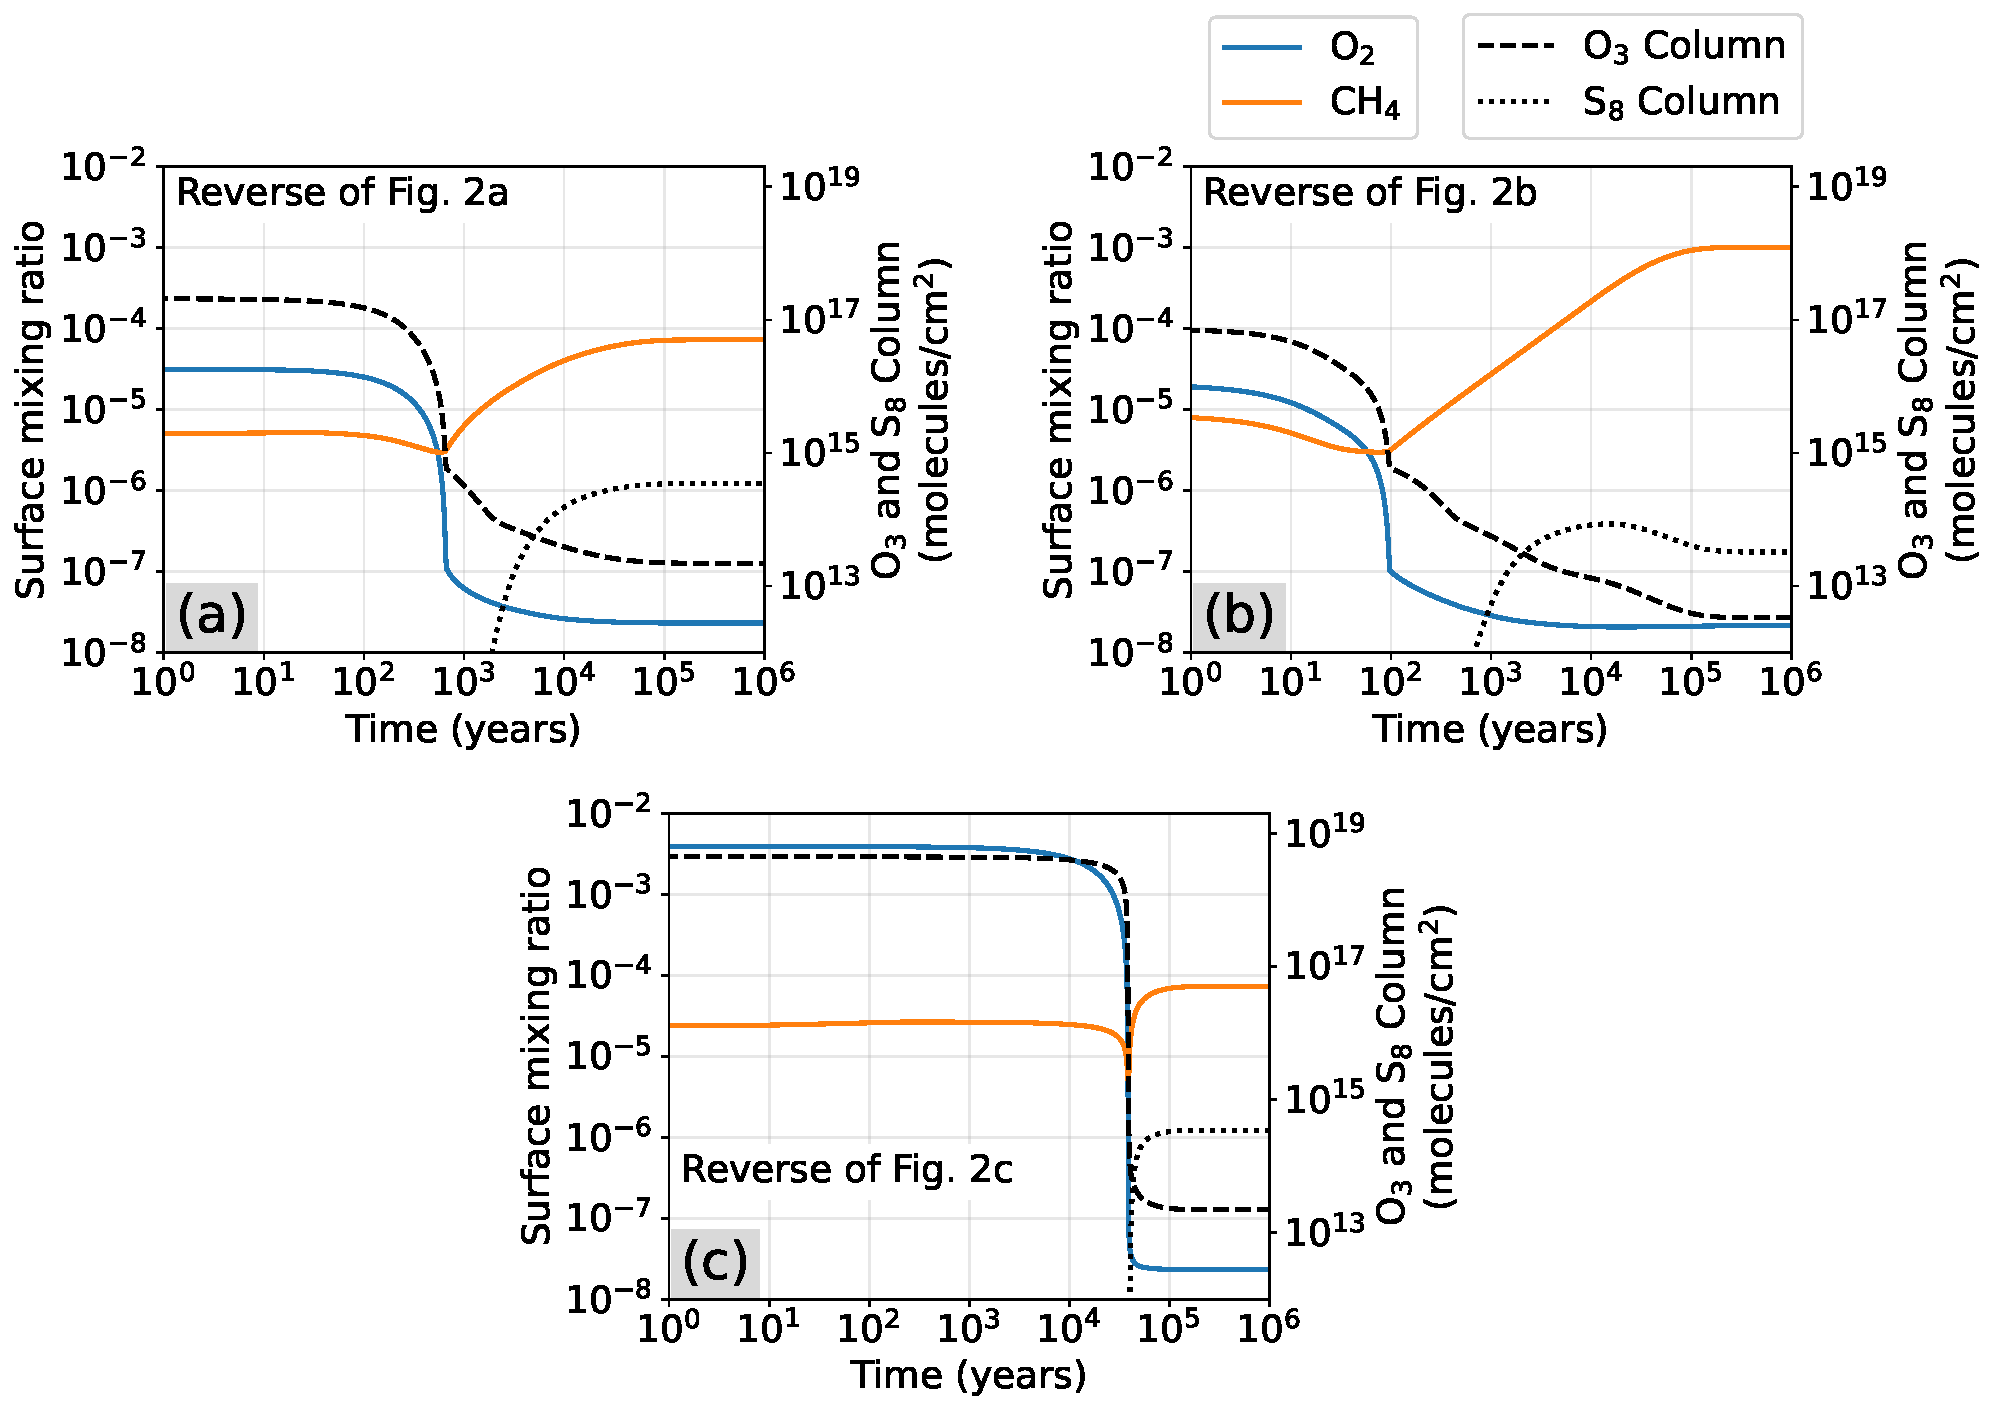
\includegraphics[width=\textwidth]{tex/4goe/main/Reversibility.pdf}
  \caption{(a), (b) and (c) show simulated reversal of the oxic transitions shown in Figures \ref{fig:oxygenation}a, \ref{fig:oxygenation}b, and \ref{fig:oxygenation}c, respectfully. Each oxic to anoxic transition is caused by a stepwise change of the CH$_4$ flux and O$_2$ flux at $t=0$ years.}
  \label{fig:reverse}
\end{figure}

Here, we use our time-dependent photochemical model to address the controversy of the reversibility of the oxic transition \citep{Poulton_2021, Izon_2022}. Figure \ref{fig:reverse}a, \ref{fig:reverse}b, and \ref{fig:reverse}c show the reverse of model runs shown in Figure \ref{fig:oxygenation}a, \ref{fig:oxygenation}b, and  \ref{fig:oxygenation}c. For each model run, we start with an atmosphere initially at a steady state at the end of the simulations shown in Figures \ref{fig:oxygenation}a - \ref{fig:oxygenation}c. Then we impose a stepwise change in the O$_2$ and CH$_4$ flux at $t = 0$ years to return the atmosphere to anoxia. The reversal of Figures \ref{fig:oxygenation}a, \ref{fig:oxygenation}b, and \ref{fig:oxygenation}c take approximately 700, 100, and 40,000 years, respectively, in comparison to the 3,500, 60,000, and the 300,000 years required for oxygenation.

Like the timescale for oxygenation, the timescale of de-oxygenation depends on the column abundance of redox sensitive gases. In the previous section, we established that the timescale required for O$_2$ to begin to rise is merely the time required to deplete the reservoirs of CH$_4$ and other reducing gases. Analogously, the timescale of deoxygenation is determined by the reservoir of O$_2$ and other oxidizing gases in the oxygenated atmosphere. The reversal shown in Figure \ref{fig:reverse}b starts with only $2 \times 10^{-5}$ O$_2$, which can be depleted very quickly, allowing the return of an anoxic atmosphere. In contrast, the reversal shown in Figure \ref{fig:reverse}c takes 40,000 years because the atmosphere starts with $4 \times 10^{-3}$ O$_2$, which takes longer to deplete. 

\subsection{The stability of post-GOE atmospheric oxygen} \label{sec:stability}

\begin{figure}
  \centering
  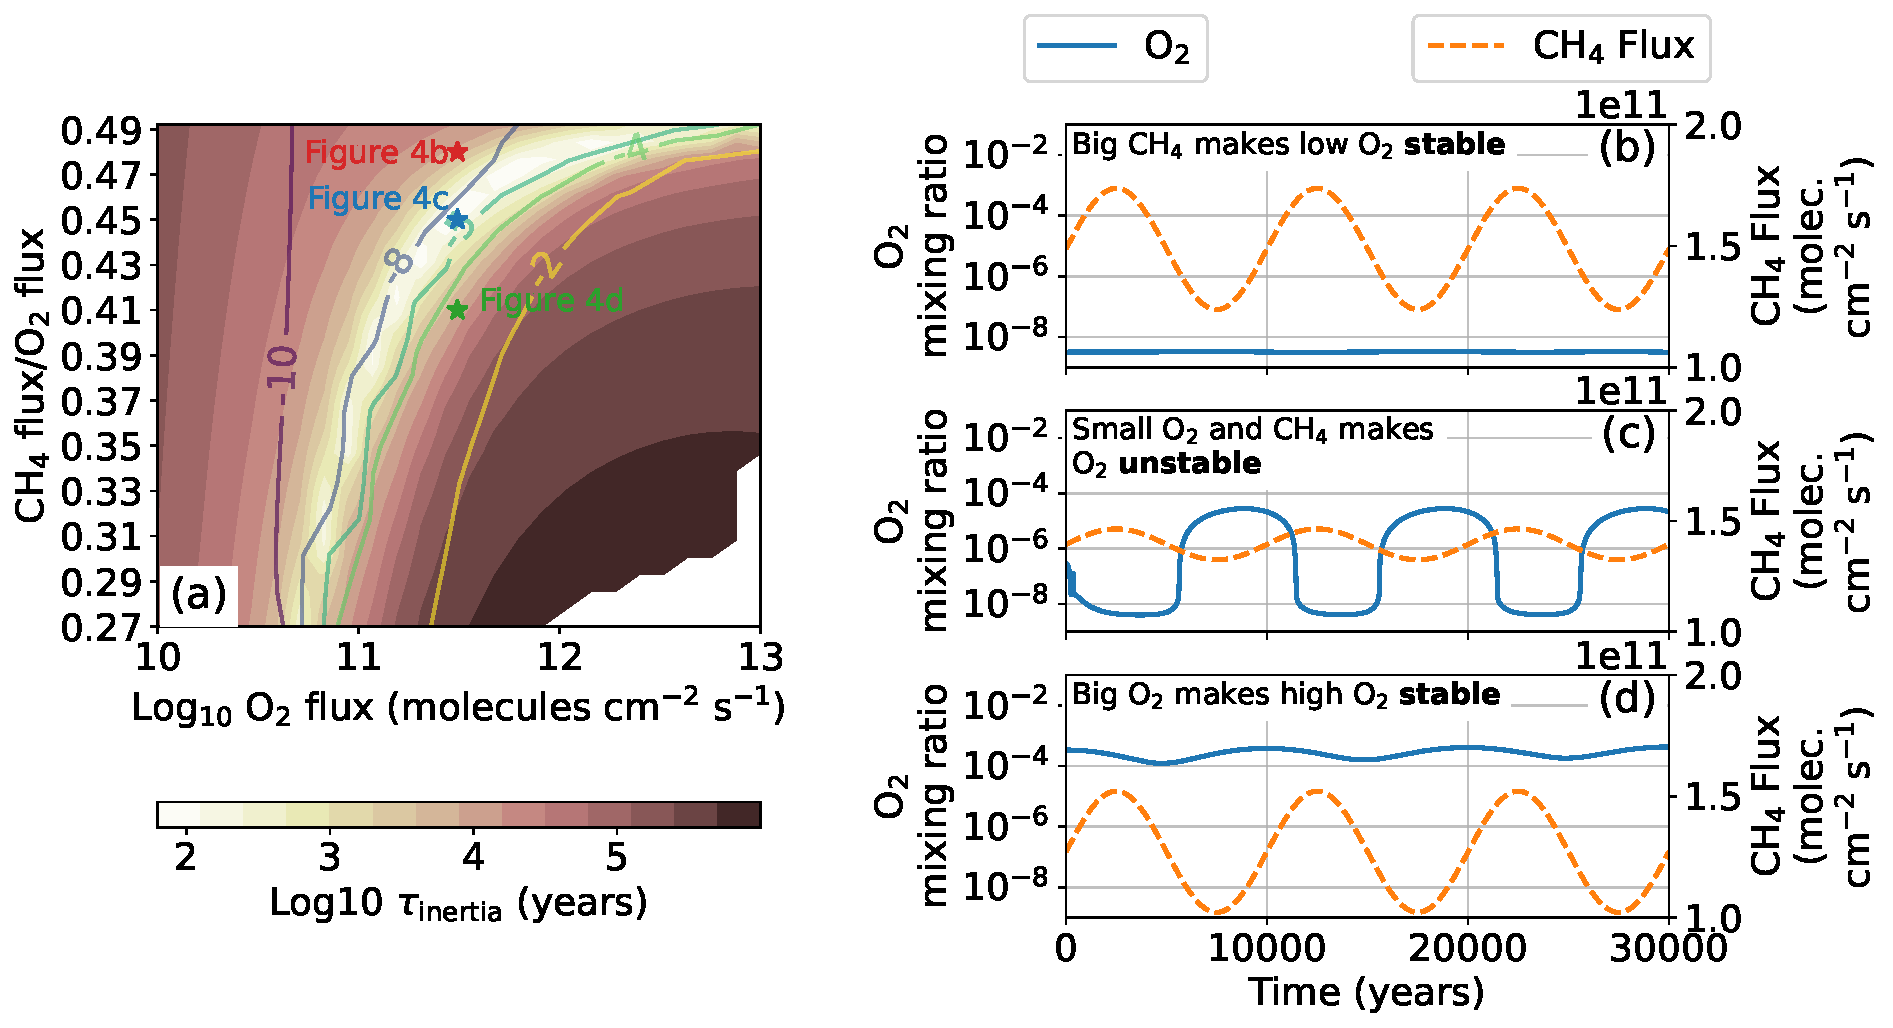
\includegraphics[width=\textwidth]{tex/4goe/main/Stability.pdf}
  \caption{The photochemical stability of O$_2$. Shading in (a) shows the steady state inertial timescale of redox gases (Equation \eqref{eq:redox_column}), and colored contours are the steady state $\log_{10}$ surface O$_2$ mixing ratio (same as Figure \ref{fig:sweep}a). (b), (c), and (d) are time-dependent photochemical simulations with oscillating CH$_4$ surface fluxes, each beginning with steady state atmospheres indicated in (a). O$_2$ stability is directly proportional to the column abundance of redox gases in the atmosphere.}
  \label{fig:stability}
\end{figure}

In the previous two sections we show that reservoirs of redox gases, primarily methane and oxygen, give the atmosphere chemical inertia, controlling the timescale of O$_2$ changes. When reservoirs are big, for similar flux perturbations, the O$_2$ mixing ratio will change relatively slowly over time; however, when reservoirs are small, photochemistry permits rapid O$_2$ transitions. Therefore, the abundance of redox gases in an atmosphere is closely linked to the photochemical stability of oxygen.

Figure \ref{fig:stability}a shows the steady state inertial timescale of redox gases, $\tau_\mathrm{inertia}$, over the same axes as Figure \ref{fig:sweep}, which shows mixing ratios. $\tau_\mathrm{inertia}$ is the sum of all redox gases in the atmospheric column (O-equivalent molecules cm$^{-2}$), divided by a characteristic flux perturbation, which we take to be 10\% of the O$_2$ flux: 

\begin{equation} \label{eq:redox_column}
  \tau_\text{inertia} = \frac{N_\mathrm{redox}}{F_\text{redox perturb.}} = \frac{\sum_i | \alpha_i | N_i}{0.1 \alpha_\mathrm{O_2} F_\mathrm{O_2}}
\end{equation}
We choose the characteristic flux perturbation to be 10\% of the O$_2$ flux because it is the same order of magnitude as natural redox variations that occur on the modern Earth during Milankovitch cycling (see the Discussion section). An upper limit for the characteristic flux perturbation would be 100\% of the O$_2$ flux. This would decrease all $\tau_\mathrm{inertia}$ values in Figure \ref{fig:stability}a by a factor of 10, which would not change our interpretation. Since CH$_4$, CO, H$_2$, and O$_2$ are the most important redox gases, the numerator in Equation \eqref{eq:redox_column} is well approximated by $4 N_\mathrm{CH_4} + N_\mathrm{CO} + N_\mathrm{H_2} + 2 N_\mathrm{O_2}$. Oxygen is the most prone to change for the smallest $\tau_\mathrm{inertia}$ values, coinciding with O$_2$ mixing ratios between $\sim10^{-8}$ and $\sim10^{-5}$ shown in the whitish region of Figure \ref{fig:stability}a.

The time-dependent photochemical models shown in Figures \ref{fig:stability}b - \ref{fig:stability}d illustrate the relationship between $\tau_\mathrm{inertia}$ and  O$_2$ instability. To produce Figure \ref{fig:stability}b, we started with the steady state atmosphere indicated on Figure \ref{fig:stability}a, then imposed 17\% amplitude oscillations to the CH$_4$ flux with a period of 10,000 years. This forcing had no perceptible effect on the $3 \times 10^{-9}$ atmospheric O$_2$. A similar 20\% CH$_4$ flux oscillations also did not significantly perturb an oxic atmosphere starting with $3 \times 10^{-4}$ O$_2$ (Figure \ref{fig:stability}d). However, just 5\% CH$_4$ flux oscillations cause $\sim4$ orders-of-magnitude oscillations in surface oxygen concentrations for an incipiently oxic atmosphere starting with $3 \times 10^{-7}$ O$_2$ (Figure \ref{fig:stability}c). O$_2$ is most unstable where the abundance of all redox gases is smallest relative to a characteristic redox surface flux (the whitish area of Figure \ref{fig:stability}a) between $\sim10^{-8}$ and $\sim10^{-5}$ O$_2$ mixing ratio. Stability continually increases outside of this range of O$_2$ concentrations.

While O$_2$ was relatively stable in the Figure \ref{fig:stability}b and \ref{fig:stability}d simulations, it does not mean these atmospheres and initial oxygen concentrations are stable to all atmospheric perturbations. The stability of any O$_2$ mixing ratio depends on the atmospheric forcings that are likely in nature. In the discussion section, we argue that the CH$_4$ flux oscillations used in Figure \ref{fig:stability} are realistic because comparable fractional changes in the methane flux have occurred over the past 650,000 years.

Flux oscillations over timescales greater than $\sim10$ years are required to significantly affect O$_2$ concentrations. Imposing 100\% amplitude fluctuations to the CH$_4$ flux with a period of 1 year, starting with the same atmosphere as Figure \ref{fig:stability}c, did not significantly alter the atmosphere over time. Atmospheres with between $\sim10^{-8}$ and $\sim10^{-5}$ O$_2$ contain some CH$_4$ and O$_2$, which gives the atmosphere inertia against annual to decadal change.

\section{Discussion} \label{sec:dis}

Recently, \citet{Bethan_2021} computed photochemical steady state atmospheres for a wide range of surface O$_2$ and CH$_4$ fluxes and found bistable O$_2$ concentrations. Their model allows steady state atmospheres for O$_2$ concentrations below $6 \times 10^{-7}$ and above $2 \times 10^{-3}$ mixing ratio but admits few steady state solutions in between. They hypothesized that feedbacks between O$_2$ and O$_3$ shielding eliminate most solutions with these intermediate O$_2$ concentrations. In contrast, our model can yield a steady state solution with intermediate O$_2$ concentrations given the right constant surface flux boundary conditions (e.g. Figure \ref{fig:oxygenation}b; see also Gregory et al. Figure 8). The difference might be caused by different steady state convergence criteria, chemical reaction networks, boundary conditions, or a combination of these factors. 

However, a photochemical steady state, e.g., at $10^{-6}$ O$_2$ mixing ratio, does not mean that such an atmosphere is stable and realistic over $10^5$ to $10^6$ year timescales. Gas fluxes from Earth's surface can vary during these timescales and significantly change O$_2$ concentrations (results section). 

For example, in the past 650,000 years, the biogenic methane flux has oscillated with an amplitude of 25\% ($6 \times 10^9$ molecules cm$^{-2}$ s$^{-1}$) and a 100,000 year period \citep{Hopcroft_2018,Spahni_2005}. On the modern Earth, methanogens in wetlands are a major source of atmospheric methane \citep{Canadell_2021}. Every 100,000 years, ice sheets have advanced and retreated, covering and uncovering wetlands, changing the CH$_4$ flux to the atmosphere. These ice ages and methane flux variations are in response to Milankovitch cycles with characteristic periods between 20,000 and 100,000 years. This exact same methane oscillation would not have occurred in the late Archean or early Proterozoic because modern wetlands did not exist then, but a similar process involving microbial mats is conceivable. 

\citet{Zhao_2018} modeled cyanobacterial mats on Proterozoic land, finding that they could have been a substantial CH$_4$ source to the atmosphere. Ice sheets covering and uncovering microbial mats could have affected global CH$_4$ fluxes. Figure \ref{fig:stability}c illustrates the effect of 5\% methane flux variations over Milankovitch timescales on an atmosphere starting with $3\times 10^{-7}$ O$_2$. O$_2$ oscillates nearly four orders of magnitude between $\sim10^{-8}$ (anoxic) and $\sim10^{-4}$ (oxic) (Figure \ref{fig:stability}).

An oscillating methane flux is only one of many possible atmospheric perturbations. The early Proterozoic geologic record preserves evidence of large igneous provinces (LIPs), or massive volcanic eruptions \citep{Gumsley_2017}. In Section \ref{sec:goe_appendix}, we show that the H$_2$ and CO outgassed from a significant LIP eruption could cause the O$_2$ surface mixing ratio to drop from $2 \times 10^{-5}$ to $4 \times 10^{-9}$ in $\sim100$ years, causing a return to sulfur isotope MIF. In this simulation, we use the maximum LIP eruption rates reported in the literature \citep{Bryan_2010}. In addition to LIPs, a Snowball Earth event concurrent with the GOE would have presumably affected gases produced by the biosphere \citep{Rasmussen_2013}.

Constant surface gas fluxes from biology and volcanism for millions of years in the aftermath of the initial rise of O$_2$ are unlikely. Additionally, our photochemical modeling shows that for atmospheres with transitional O$_2$ concentrations, relatively small atmospheric perturbations (e.g. a CH$_4$ flux change of 5\%) over timescales as short as 100s of years can cause O$_2$ to change by orders of magnitude (e.g. Figure \ref{fig:reverse}b). Therefore, substantial variability of O$_2$ during the GOE appears possible.

For these reasons, our photochemical modeling results are compatible with recently published evidence of fluctuating sulfur isotope MIF \citep{Poulton_2021, Gumsley_2017} indicating that O$_2$ was unstable between 2.4 and 2.2 Ga. We find that shut-off of S$_8$ aerosol production, which is required to produce sulfur isotope MIF, occurs at $\sim10^{-7}$ O$_2$ mixing ratio, a region of the parameter space where O$_2$ is prone to rapid change (Figure \ref{fig:stability}). But, oxygen surface levels between $\sim10^{-8}$ and $\sim10^{-4}$ mixing ratio were likely unstable. Short period changes to the biosphere, or volcanic outgassing rates could have caused order of magnitude O$_2$ changes over 100 to 100,000 year timescales. Occasionally, big perturbations to the atmosphere, such as a LIP, might have lowered O$_2$ concentrations enough for sulfur isotope MIF to reoccur. Note, the above explanation for the cause of O$_2$ oscillations prior to 2.2 Ga is complicated by S-MIF data presented in \citet{Izon_2022}, which do not suggest the same O$_2$ variability found by \citet{Poulton_2021}.

After 2.2 Ga, and during the mid-Proterozoic, sulfur isotope MIF never returned. Therefore, this time must have had O$_2$ concentrations large enough to prevent O$_2$ collapse. Our modeling shows that larger O$_2$ concentrations give the atmosphere chemical inertia, slowing atmospheric deoxygenation (Figure \ref{fig:reverse}). It is therefore challenging to reconcile our modeling results with the interpretation of \citet{Planavsky_2014_proto}, who used Proterozoic chromium isotopes to argue that O$_2$ could not have been larger than $2 \times 10^{-4}$ mixing ratio. Such a small O$_2$ reservoir would have been unstable to LIP eruptions, or variations in the CH$_4$ flux from Milankovitch cycles (Figure \ref{fig:stability}), which both have evidence for occurring in the mid-Proterozoic stratigraphic record \citep{Zhang_2015,Meyers_2018,Lecheminant_1989}. We conclude that for stability, mid-Proterozoic O$_2$ levels should have exceeded $\sim 10^{-4}$. This conclusion is compatible with mid-Proterozoic Fe isotopes in ironstones, which suggest O$_2$ levels between approximately $2 \times 10^{-4}$ - $2 \times 10^{-3}$ mixing ratio \citep{Wang_2022}.

Our results are not sensitive to the changing solar UV photon flux between the GOE ($\sim 2.4$ Ga) and the mid-Proterozoic. Re-calculating Figure \ref{fig:sweep} using the solar UV flux at 1.3 Ga \citep{Claire_2012} results in surface O$_2$ and CH$_4$ surface mixing ratios within a factor of 2 of Figure \ref{fig:sweep}.

Our work also has implications for the most likely oxygen levels before the GOE. \citet{Johnson_2021} analyzed molybdenum isotopes in the Archean sedimentary record for signs of continental oxidative weathering. Their work is compatible with two end-member interpretations: (1) if Archean O$_2$ was evenly distributed over the globe, then the surface O$_2$ mixing ratio was $> 3 \times 10^{-8}$ and $< 2 \times 10^{-7}$, or (2) if O$_2$ accumulation was geographically restricted, then the O$_2$ surface flux was greater than 0.01 Tmol yr$^{-1}$ ($3 \times 10^{7}$ molecules cm$^{-2}$ s$^{-1}$). Our modeling suggests (1) is unlikely because we find that O$_2$ is likely unstable over geologic time for this range of oxygen levels.

In our modeling, we do not explicitly consider redox reservoirs in the oceans, sediments, crust, and mantle for good reason. These reservoirs are coupled to the atmosphere and can modulate O$_2$ levels. However, the timescale of equilibration between the atmosphere and other redox reservoirs is often relatively long (e.g. 100 Myr for organic carbon in continental sediments), so we consider them to be approximately constant over the timescale of O$_2$ transitions ($<10^5$ years).

A caveat is the coupling between redox reservoirs in the atmosphere, crust or sediments might depend on atmospheric composition. An example is the pyrite oxidation rate, which depends on the partial pressure of oxygen \citep{Bethan_2021}. We do not explicitly consider such feedbacks, which could affect the timescale of changing O$_2$ levels.

An additional, related caveat is that our model does not consider biological feedbacks. The rise of O$_2$ would limit habitats for anaerobes, and permit more widespread aerobic respiration, potentially dropping the CH$_4$ flux / O$_2$ flux ratio further than we have modeled here. Also, a stronger ozone UV shield would make new habitats for cyanobacteria and allow the expansion of life on land, promoting chemical and oxidative weathering. All these changes, which we do not explicitly model, would modulate oxygen levels. In this article, we impose changes in the CH$_4$ and O$_2$ flux that are suppose to be representative of a changing biosphere, but a better model would determine more realistic changes in gas fluxes by directly coupling 1-D photochemistry and biology.

\section{Conclusions}

Our time-dependent photochemical modeling of the Great Oxidation Event suggests that oxygen can rise and fall over geologically short periods of time. For an anoxic to oxic transition, once a tipping point of imbalanced redox fluxes is reached, the reservoir of reducing gases in the atmosphere must be eliminated before O$_2$ can begin to rise. This takes 100s to 10,000s of years. O$_2$ accumulation to just hundredths or tenths of percent levels requires filling a large O$_2$ reservoir, which may occur on a $10^5$ year timescales. Atmospheric de-oxygenation occurs over similar periods of time, mainly controlled by the magnitude of the initial O$_2$ abundance.

We also find O$_2$ instability, especially for mixing ratios between $\sim10^{-8}$ and $\sim10^{-5}$. For these O$_2$ concentrations, photochemistry demands that both CH$_4$ and O$_2$ be relatively small in concentration. This small reservoir of redox sensitive gases permits rapid changes to the atmosphere’s redox state. For example, for an atmosphere starting with $3 \times 10^{-7}$ O$_2$, 5\% amplitude oscillations to the methane flux with a period of 10,000 years cause oxygen to fluctuate four orders of magnitude between anoxic and oxic. Additionally, we show that a LIP eruption could cause the collapse of O$_2$ and the return of sulfur isotope MIF for an atmosphere starting with $2 \times 10^{-5}$ O$_2$ mixing ratio (Supporting Information).

We emphasize that the short term ($10^2$ - $10^5$ year) variability in O$_2$ levels considered here occurred on the backdrop of the billion year oxidation of the crust and mantle, and long-term organic burial, which are argued to be the ultimate causes of the rise of oxygen on Earth \citep[e.g.][]{Catling_2001}.

Overall, our modeling is compatible with, but does not prove, proposed geologic evidence for fluctuating and unstable atmospheric O$_2$ after the initial rise of oxygen 2.4 billion years ago. A single, uni-directional, oxidation event remains plausible, although would require strong and perhaps biological feedbacks promoting permanent substantial changes in the global CH$_4$ flux / O$_2$ flux ratio. While this is evident between the Archean (CH$_4$ flux / O$_2$ flux $\sim 0.5$) and modern (CH$_4$ flux / O$_2$ flux $\sim 0.1$) biospheres, the dynamics of the Proterozoic biosphere remain largely unexplored. Also, our results suggest that a stable, post-GOE, mid-Proterozoic atmosphere would need an O$_2$ mixing ratio exceeding a value in the $10^{-4}$ - $10^{-3}$ range. 

\section{Chapter Appendix} \label{sec:goe_appendix}

\subsection{Photochemical modeling details}

All Great Oxidation Event (GOE) simulations use the solar spectrum at 2.4 Ga, calculated with methods described in \citet{Claire_2012}. We also always include chemical rainout and NO production from lightning. 95\% of steady state simulations conserve redox to a factor better than $10^{-6}$. 3\% of models, all with $> 0.1\%$ steady-state O$_2$, conserve redox to a factor of $\sim10^{-3}$. Figure \ref{fig:case1} shows results from steady-state photochemical simulations over the same parameter space as Figure \ref{fig:sweep}, except using the ``Modern Values'' fluxes from Table \ref{tab:volc_fluxes}. Figure \ref{fig:eddy_temp} shows assumed eddy diffusion and temperature profiles. 

\begin{figure}
  \centering
  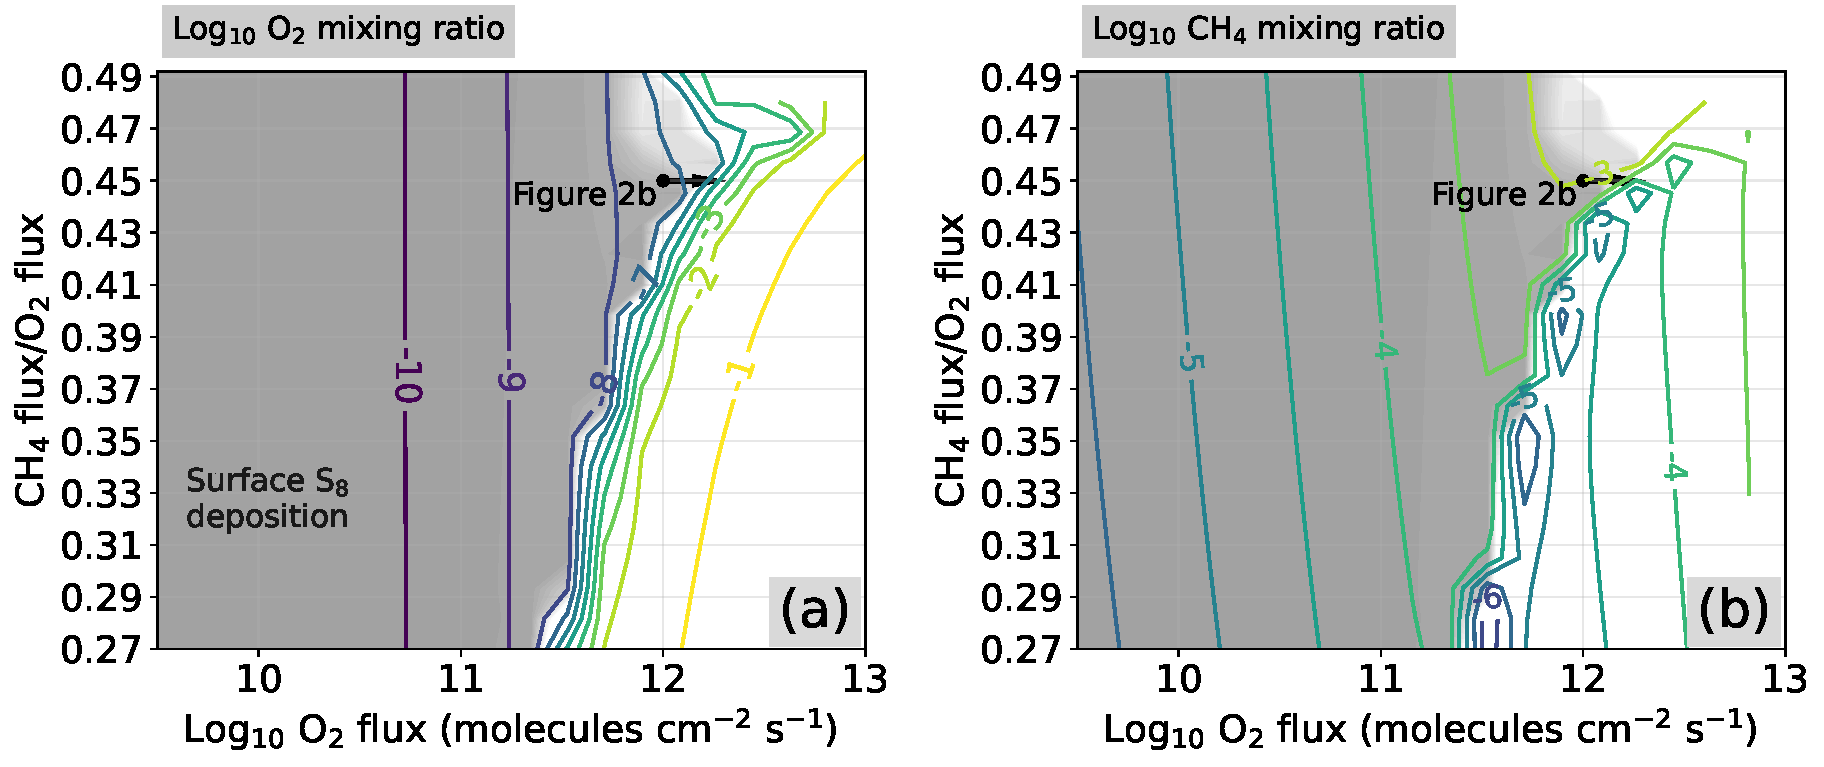
\includegraphics[width=\textwidth]{tex/4goe/supplement/figures/ModernValues_sweep.pdf}
  \caption{Identical to Figure \ref{fig:sweep}, except we use the ``Modern Values'' surface fluxes in Table \ref{tab:volc_fluxes}. The time-dependent photochemical simulation shown in Figure \ref{fig:oxygenation}b, is indicated with a black arrow.}
  \label{fig:case1}
\end{figure}
  
\begin{figure}
  \centering
  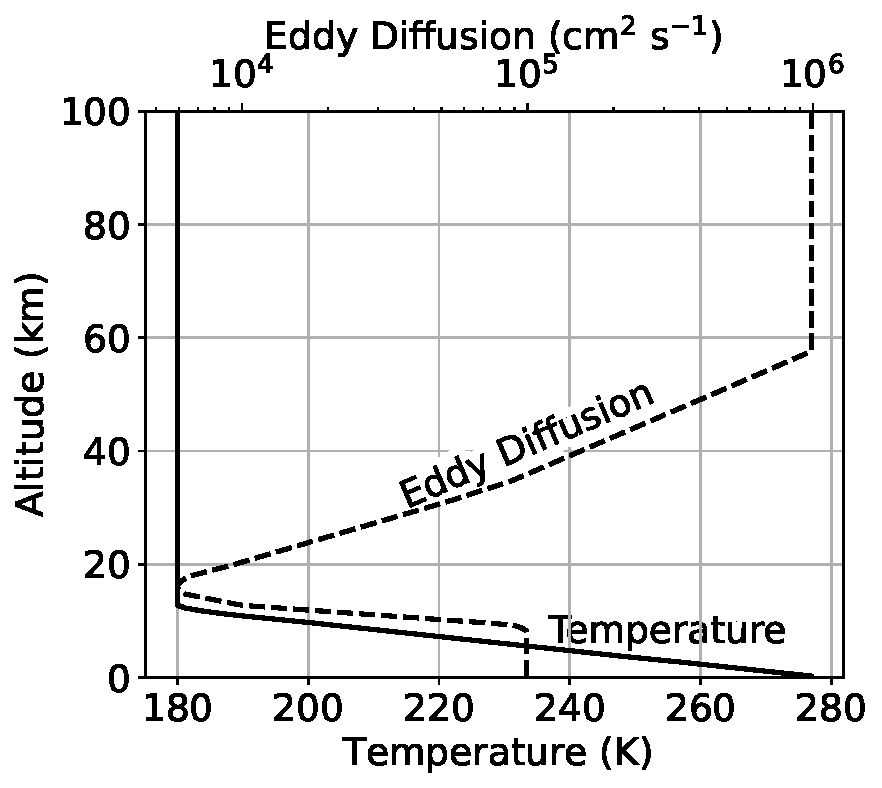
\includegraphics[width=0.5\textwidth]{tex/4goe/supplement/figures/A1_temp_eddy.pdf}
  \caption{The temperature and eddy diffusion used for every simulation.}
  \label{fig:eddy_temp}
\end{figure}

\subsection{Estimating the timescale of the rise of O\textsubscript{2}}

In Section \ref{sec:goe_results}, we estimated the timescale for the rise of O$_2$ using the following equation:

\begin{equation} \label{eq:tau_oxy_SI}
    \tau_\text{oxy} = \left| \frac{\Delta N_\text{reducing}}{\Delta F_\mathrm{O_{equiv}}} \right|
\end{equation}
Applying this equation to the Figure \ref{fig:oxygenation}b simulation:

\begin{equation}
\begin{split}
\Delta F_\mathrm{O_{equiv}} &= (2 F_\mathrm{O_2}^\text{final} - 4 F_\mathrm{CH_4}^\text{final}) - (2 F_\mathrm{O_2}^\text{initial} - 4 F_\mathrm{CH_4}^\text{initial}) \\
&= (2(1.8\times10^{12}) - 4(8.1\times10^{11})) - (2(1.0\times10^{12}) - 4(4.5\times10^{11})) \\
&= 1.6 \times 10^{11} \:\mathrm{molecules}\:\mathrm{cm^{-2}}\:\mathrm{s^{-1}}
\end{split}
\end{equation}

\begin{equation} \label{eq:tau_oxy_case1}
    \tau_\text{oxy} = \left| \frac{\Delta N_\text{reducing}}{\Delta F_\mathrm{O_{equiv}}} \right| = \left|\frac{1.47 \times 10^{23}} {1.6 \times 10^{11}} \right| = 9.8 \times 10^{11} \: \text{s} = 29,000 \: \text{years}
\end{equation}
This estimation is about a factor of two smaller than the $\sim$60,000 years predicted by our time-dependent photochemical model. 

Figure \ref{fig:column_rate} shows the column of reducing gases and its destruction rate during the Figure \ref{fig:oxygenation}b simulation. Our estimation for the timescale of oxygenation (Equation \eqref{eq:tau_oxy_case1}) is off by a factor of two because the reducing column evolves over time, and our estimation of its destruction rate ($\Delta F_\mathrm{O_{equiv}}$) is too large. In the photochemical model, chemistry and transport does not permit a reducing column destruction rates identical to the imposed change in redox fluxes at the surface ($1.6 \times 10^{11}$ O molecules cm$^{-2}$ s$^{-1}$).

\begin{figure}
  \centering
  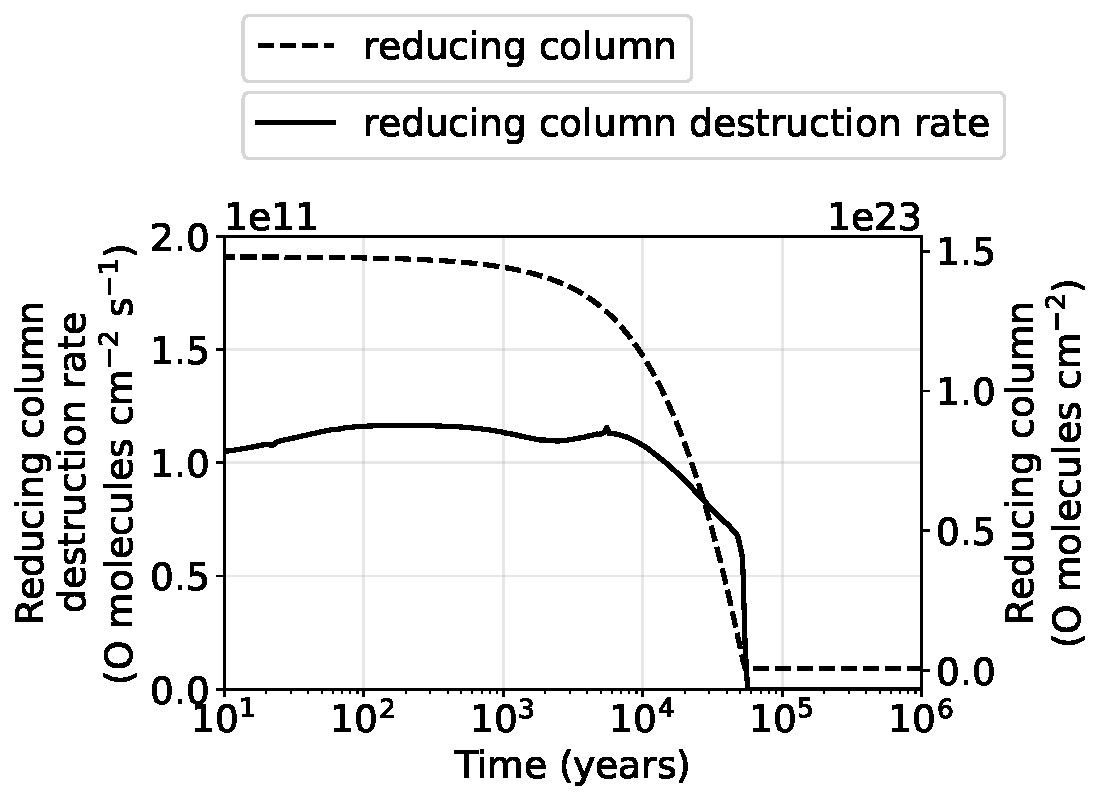
\includegraphics[width=0.7\textwidth]{tex/4goe/supplement/figures/Column_rates.pdf}
  \caption{Reducing gas column and its destruction rate for the simulation shown in Figure \ref{fig:oxygenation}b.}
  \label{fig:column_rate}
\end{figure}

\subsection{A Large Igneous Province may have destabilized atmospheric oxygen}

Here, we show that the H$_2$ and CO outgassing from large igneous provinces (LIPs), or massive volcanic eruptions, could have potentially caused the collapse of transitional O$_2$ concentrations ($\sim 10^{-8}$ to $\sim 10^{-4}$ mixing ratio). 

To compute H$_2$ and CO outgassing rates from LIPs, we use the outgassing model described in \citet{Wogan_2020_methane}. To briefly summarize, the model estimates the composition of gas bubbles suspended in magma just prior to release into the overlying atmosphere or ocean. Gas composition is computed by solving a system of equations including solubility relationships for H$_2$O and CO$_2$, gas-phase equilibrium relationships, and mass conservation of hydrogen and carbon. The model has five inputs: Magma oxygen fugacity, temperature, and overburden pressure, and the H$_2$O and CO$_2$ mass fractions ($m_\mathrm{H_2O}^\mathrm{tot}$, and $m_\mathrm{CO_2}^\mathrm{tot}$) in the magma before degassing occurs. For LIPs, we assume a magma oxygen fugacity one log-unit below the fayalite-magnetite-quartz mineral redox buffer (i.e. $\Delta$FMQ-1) following Archean proxies \citep{Aulbach_2016}. See Chapter 7 in \citet{Catling_2017} for a description of the fayalite-magnetite-quartz redox buffer. Additionally, we use $m_\mathrm{H_2O}^\mathrm{tot} = 0.5$ wt\% and $m_\mathrm{CO_2}^\mathrm{tot} = 0.05$ wt\% which agrees with estimates of LIP volatile concentrations \citep{Wallace_2015}. Finally, we take the degassing temperature and pressure to be 1473 K and 1 bar, respectfully. With these inputs, our outgassing model predicts $1.6 \times 10^{-2}$ mol H$_2$/kg magma and $1.7 \times 10^{-3}$ mol CO/kg magma. 

Converting gas production rates (e.g. mol H$_2$/kg magma) into gas fluxes to the atmosphere requires estimations of magma eruption rates during LIPs. Basaltic LIPs typically last several million years and cumulatively produce $>3 \times 10^{18}$ kg magma \citep{Self_2015}. This magma is release over 10s to 100s of eruptions each lasting several years to 10s of years with eruptions rates between $3 \times 10^{13}$ to $3 \times 10^{15}$ kg magma yr$^{-1}$ \citep{Bryan_2010}. Multiplying these eruption rates by calculated gas production yields H$_2$ fluxes between $1.9 \times 10^9$ and $1.9 \times 10^{11}$ molecules cm$^{-2}$ s$^{-1}$ and CO fluxes between $2.0 \times 10^8$ and $2.0 \times 10^{10}$ molecules cm$^{-2}$ s$^{-1}$. 

The time-dependent photochemical simulation shown in Figure \ref{fig:volc} shows how atmospheric O$_2$ responds to maximum LIP H$_2$ and CO outgassing scenario. The simulation starts with an atmosphere initially at equilibrium, then at $t = 0$ years, we increase the H$_2$ and CO outgassing fluxes by $1.9 \times 10^{11}$ and $2.0 \times 10^{10}$ molecules cm$^{-2}$ s$^{-1}$, respectfully. O$_2$ drops from $2 \times 10^{-5}$ to $4 \times 10^{-9}$ in 100 years. Basaltic LIP eruptions can last for 10s of years \citep{Bryan_2010}, so a 100 year eruption, which is required to cause O$_2$ to collapse, is within the realm of possibility. However, the period of anoxia would likely be maintained for only a few hundred years, until the eruption ceased. Several periods of anoxia, each corresponding to a significant eruption, might occur during an entire several-million-year LIP event.

\begin{figure}
  \centering
  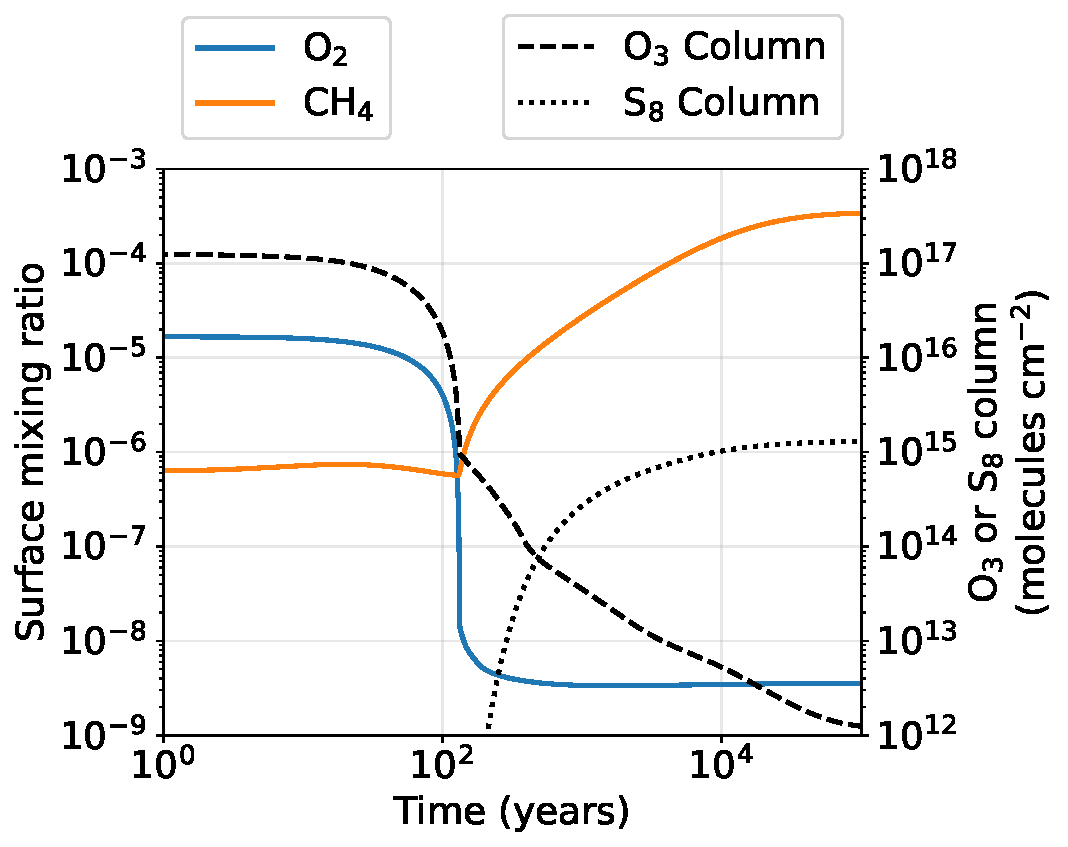
\includegraphics[width=0.7\textwidth]{tex/4goe/supplement/figures/Volcanism.pdf}
  \caption{Modeled oxic to anoxic transition caused by H$_2$ and CO outgassing from a large igneous province eruption. The simulation begins with a photochemical equilibrium atmosphere, and then is perturbed by a stepwise increase of the H$_2$ and CO flux by $1.9 \times 10^{11}$ and $2.0 \times 10^{10}$ molecules cm$^{-2}$ s$^{-1}$, respectfully. A LIP eruption should able to produce these outgassing fluxes for the 100 years required to cause O$_2$ to collapse (see text).}
  \label{fig:volc}
\end{figure}

It is unclear whether a 100 year period of anoxia is detectable in the geologic record of multiple sulfur isotopes. A single sample from the sedimentary record might represent a period of time greater than 100 years, thus containing sulfur from both an oxic and anoxic atmosphere, diluting the S-MIF signal. Evaluating the detectability of short-term anoxia in the sedimentary record of sulfur isotopes is an interesting target for future work coupling in-situ and bulk rock measurements \citep{Meyer_2017}.

LIPs may have additional effects on the atmosphere that we are not accounting for in the above calculations. For example, increased Cl outgassing could catalyze O$_3$ and CH$_4$ destruction (e.g. $\mathrm{Cl} + \mathrm{O_3} \rightarrow \mathrm{ClO} + \mathrm{O_2}$ and $\mathrm{Cl} + \mathrm{CH_4} \rightarrow \mathrm{HCl} + \mathrm{CH_3}$), which could have a non-trivial effect on the O$_2$ concentration.